
\documentclass[a4paper,12pt]{article} % This defines the style of your paper

\usepackage[top = 2.5cm, bottom = 2.5cm, left = 2.5cm, right = 2.5cm]{geometry} 

% fonts
\usepackage[T1]{fontenc}
\usepackage[utf8]{inputenc}
\usepackage{xcolor}
\usepackage{amsmath}
\usepackage{amsfonts}
\usepackage{amssymb}
\usepackage{enumitem}
\usepackage{mathtools}
   
% The following two packages - multirow and booktabs - are needed to create nice looking tables.
\usepackage{multirow} % Multirow is for tables with multiple rows within one cell.
\usepackage{booktabs} % For even nicer tables.

% The default setting of LaTeX is to indent new paragraphs. This is useful for articles. But not really nice for homework problem sets. The following command sets the indent to 0.
\usepackage{setspace}
\setlength{\parindent}{0in}

% Package to place figures where you want them.
\usepackage{float}

% The fancyhdr package let's us create nice headers.
\usepackage{fancyhdr} 


%%%%%%%%%%%%%%%%%%%%%%%%%%%%%%%%%%%%%%%%%%%%%%%%
% Header (and Footer)
%%%%%%%%%%%%%%%%%%%%%%%%%%%%%%%%%%%%%%%%%%%%%%%%

\pagestyle{fancy} % With this command we can customize the header style.

\fancyhf{} % This makes sure we do not have other information in our header or footer.

\lhead{\footnotesize Numerics for SDE}% \lhead puts text in the top left corner. \footnotesize sets our font to a smaller size.
\newtheorem{proposition}{Proposition}

%\rhead works just like \lhead (you can also use \chead)
\rhead{\footnotesize Alvise Sembenico}%, Lastname 2 (\& Lastname 3)} %<---- Fill in your lastnames.

% Similar commands work for the footer (\lfoot, \cfoot and \rfoot).
% We want to put our page number in the center.
\cfoot{\footnotesize \thepage} 
\newcommand{\Var}{\mathrm{Var}}
\newcommand{\Cov}{\mathrm{Cov}}


%%%%%%%%%%%%%%%%%%%%%%%%%%%%%%%%%%%%%%%%%%%%%%%%
% Custom commands
\newcommand{\comment}[1]{%
  \text{\phantom{(#1)}} \tag{#1}
}
%%%%%%%%%%%%%%%%%%%%%%%%%%%%%%%%%%%%%%%%%%%%%%%%

%%%%%%%%%%%%%%%%%%%%%%%%%%%%%%%%%%%%%%%%%%%%%%%%
% Document
%%%%%%%%%%%%%%%%%%%%%%%%%%%%%%%%%%%%%%%%%%%%%%%%
\begin{document}
\begin{center} % Everything within the center environment is centered.
    {\Large \bf Homework 1}
\end{center}

\vspace{0.4cm}

%%%%%%%%%%%%%%%%%%%%%%%%%%%%%%%%%%%%%%%%%%%%%%%%
% THE HOMEWORK
% Can be written right here or in the dedicated files
%%%%%%%%%%%%%%%%%%%%%%%%%%%%%%%%%%%%%%%%%%%%%%%%

\onehalfspacing
\section{Exercise 1}
The so defined time inversion process

\begin{equation}
    B(t, \alpha) = \begin{cases}
        t^{\alpha} W(1/t) & t > 0 \\
        0                 & t = 0
    \end{cases}
\end{equation}

in order to be a Brownian Motion has to satisfy the following properties:
\begin{enumerate}
    \item with probability 1, the mapping \( t \mapsto W(t) \) is continuous and \( W(0) = 0 \);
    \item if \( 0 = t_0 < t_1 < \cdots < t_N = T \), then the increments
          \[
              W(t_N) - W(t_{N-1}), \dots, W(t_1) - W(t_0)
          \]
          are \textit{independent}; and
    \item for all \( t > s \) the increment \( W(t) - W(s) \) has the \textit{normal} distribution, with \( E[W(t) - W(s)] = 0 \) and \( E[(W(t) - W(s))^2] = t - s \)
\end{enumerate}

We begin by verifying property (1). It's clear from the property of the Brownian Motion \(W\) that \(B(t, \alpha )\) is continuous in \((0, \infty )\). The only point that we need to check the continuity is in fact at \(t=0\).

As the hint suggests, we start by computing the following for an arbitrary \(h>0, t>0\).
\begin{align*}
    \Cov\left[B(t+h, \alpha), B(t, \alpha)\right]
     & = \mathbb{E} \left[ (t+h)^{\alpha} t^{\alpha} W\left( \frac{1}{t} \right) W\left( \frac{1}{t+h} \right) \right] - \mathbb{E} \left[ B(t+h, \alpha) \right] \mathbb{E} \left[ B(t, \alpha) \right].
\end{align*}
We note that \( \mathbb{E} \left[ B(t, \alpha) \right] = t^{\alpha }\mathbb{E} \left[ W\left( \frac{1}{t} \right)  \right]=0 \). Thus, the right hand side can be simplified as follows.

\begin{align*}
    \Cov\left[B(t+h, \alpha ), B(t, \alpha ) \right] & = \mathbb{E} \left[ (t+h)^{\alpha} t^{\alpha} W\left( \frac{1}{t} \right) W\left( \frac{1}{t+h} \right) \right] \\
                                                     & = (t+h)^{\alpha } t^{\alpha } \frac{1}{t+h}                                                                     \\
                                                     & = (t+h)^{\alpha -1} t^{\alpha }
\end{align*}
Where in the one to last equality we used the fact that \(\mathbb{E} \left[ W_s W_t \right]= \min (s,t)\).
This gives a necessary condition for \(B(t, \alpha )\) to be a Brownian Motion, that is \(\alpha =1\).
We will proceed in showing the other properties of \(B(t, \alpha )\) assuming \(\alpha =1\).

For a mesh \(\Pi  = t_1 <t_2<\dots <t_n\) we write the process \(B_t\) as follows.

\begin{equation}
    \begin{bmatrix}
        B(t_1) \\
        \vdots \\
        B(t_n)
    \end{bmatrix}
    = A
    \begin{bmatrix}
        W\left( \frac{1}{t_1} \right) \\
        \vdots                        \\
        W\left( \frac{1}{t_n} \right)
    \end{bmatrix}
\end{equation}
Where just by the definition of the process \(B_t\), we have \(A = \mathrm{diag} (t_1, \dots ,t_n)\).
Moreover, we can write the matrix on the right hand side as follows
\begin{equation}
    \begin{bmatrix}
        W\left( \frac{1}{t_1} \right) \\
        \vdots                        \\
        W\left( \frac{1}{t_n} \right)
    \end{bmatrix}
    = O^n +
    \begin{bmatrix}
        \frac{1}{\sqrt{t_1}} \\
        \vdots               \\
        \frac{1}{\sqrt{t_n}}
    \end{bmatrix}
    \begin{bmatrix}
        \mathcal{N}(0, 1) \\
        \vdots            \\
        \mathcal{N}(0, 1)
    \end{bmatrix}.
\end{equation}
Upon defining the matrix \(D^n \) as follows

\begin{equation}
    D^n =
    \begin{bmatrix}
        0 & \cdots  & 0 \\
          & I_{n-1} &
    \end{bmatrix}.
\end{equation}
We can then write the matrix of the increments with the ingredients we have prepared so far.

\begin{equation}B^{\prime} =
    \begin{bmatrix}
        B_{t_1} \\
        \vdots  \\
        B_{t_n}
    \end{bmatrix}
    -
    \begin{bmatrix}
        0      \\
        B_1    \\
        \vdots \\
        B_{t_{n-1}}
    \end{bmatrix}
\end{equation}
It follows that \(B^{\prime} = A \mathcal{W}- D^{n}A \mathcal{W}  =(I-D^n)A \mathcal{W} \), where \(\mathcal{W} = \begin{bmatrix}
    W\left( \frac{1}{t_1} \right) \\
    \vdots                        \\
    W\left( \frac{1}{t_n} \right)
\end{bmatrix}\).
From this representation we get that \(B^{\prime} \) is a multivariate Gaussian Since, implying that each marginal is also Gaussian.
Moreover, we have that \(\mathbb{E} \left[ B_{t_n}- B_{t_{b_{n-1}}} = 0  \right]\). Moreover, we have that
\begin{align*}
    \Cov\left[B^{\prime}_i, B^{\prime} _j \right]
     & = \mathbb{E} \left[ B_{i}^{\prime}B^{\prime} _j   \right]                                                                                                                                                                                                                                                                                                                       \\
     & = \mathbb{E} \left[ \left( W\left( \frac{1}{t_i} \right) - W\left( \frac{1}{t_{i-1}} \right) \right) \left( W\left( \frac{1}{t_j} \right) - W\left( \frac{1}{t_{j-1}} \right) \right) \right]                                                                                                                                                                                   \\
     & = \mathbb{E} \left[ W\left( \frac{1}{t_i} \right) W\left( \frac{1}{t_j} \right) \right] - \mathbb{E} \left[ W\left( \frac{1}{t_i} \right) W\left( \frac{1}{t_{j-1}} \right) \right] - \mathbb{E} \left[ W\left( \frac{1}{t_{i-1}} \right) W\left( \frac{1}{t_j} \right) \right] + \mathbb{E} \left[ W\left( \frac{1}{t_{i-1}} \right) W\left( \frac{1}{t_{j-1}} \right) \right] \\
     & = 0
\end{align*}

From the previous point, by taking the limit of the mesh \(\mathcal{P}\), we have that for every \(a_t\) and \(t \in  [0, \infty ) \cap \mathbb{Q}\), the following holds true: \(P(\{ B(t) <a_t , a_t \in  \mathbb{R},t \in  [0, \infty ) \cap \mathbb{Q} \} ) = P(\{ B(t) <a_t , a_t \in  \mathbb{R},t \in  [0, \infty ) \cap \mathbb{Q} \} )\).
To conclude the proof that \(B\) is continuous at \(t=0\) we use the following proposition.
\begin{proposition}
    Let \((x_n)_{n \in  \mathbb{Q}}\) with \(x_n \to 0\) and let \( X(x_n) \xrightarrow{d} Y(x_n) \), \( Y(x_n) \to c \) a.s.. Then, \( X(x_n) \to c \) a.s..
\end{proposition}



\section{Exercise 2}
\subsection{}
In this exercise we will prove the following equality:
\begin{equation}
    \int_0^T t \, dW(t) = T W(T) - \int_0^T W(t) \, dt
\end{equation}
Look at the left hand side, by taking it's forward Euler we obtain
\begin{equation}
    I_1 = \int _0^T t dW(t) = \sum_{n=0}^{N-1} t_n (W(t_{n-1} -W(t_n) )).
\end{equation}
Applying the hint, i.e. using the Abel's summation by parts we get
\begin{align*}
    \sum_{n=0}^{N-1} t_n (W(t_{n-1} -W(t_n) )) & = t_N W(t_N) - t_0 W(t_0) - \sum_{k=1}^{N-1} W(t_k) (t_k - t_{k-1}) \\
                                               & = T W(T)  - \sum_{k=1}^{N-1} W(t_k) (t_k - t_{k-1}).
\end{align*}
What is left to prove is the convergence in \(L_2\) of the right hand side, i.e. the following equation.
\begin{equation}
    \lim_{n \to \infty} \mathbb{E} \left[ \left(   \int _0^T W(t)dt-\sum_{k=1}^{N-1} W(t_k) (t_k - t_{k-1})  \right)^2\right] =0.
\end{equation}
Let's fix \(t_n - t_{n-1} = \Delta t\) for every \(n\geq 0\).
Using the linearity of the integral, we can rewrite it as follows
\begin{align*}
    \mathbb{E} \left[ \left( \sum_{n=0}^{N-1}  \int _{t_{n-1}}^{t_n} W(t)dt-\sum_{k=1}^{N-1} W(t_k) (t_k - t_{k-1}) \right) ^2  \right] & = \mathbb{E} \left[ \left(   \sum_{n=0}^{N-1}  \int _{t_{n-1}}^{t_n} W(t)-W(t_n)dt  \right)^2 \right] \\
                                                                                                                                        & =\sum_{n=0}^{N-1} \mathbb{E} \left[  \int _{t_{n-1}}^{t_n} W(t)-W(t_n) dt \right]                     \\
                                                                                                                                        & = \sum_{n=0}^{N-1} \mathbb{E} \left[  e_n ^2 \right].
\end{align*}
Where \(e_n\) is n-th error term. Moreover, in the last equation we dropped the cross terms  since \(\mathbb{E} \left[ e_i e_j \right] = 0 \) by the properties of the Brownian motion.

Next, we compute \(\mathbb{E} \left[ e_n^2 \right]\) for every \(n \geq 0\).

\begin{align*}
    \mathbb{E} \left[ e_n^2 \right] & = \mathbb{E} \left[ \left(  \int _{t_n}^{t_{n-1}} W(t)- W(t_n)dt  \right)^2\right]                                                         \\
                                    & = \mathbb{E} \left[  \int _{t_n}^{t_{n-1} } \int _{t_n}^{t_{n-1} } \left( W(t)-W(t_n)dt \right)\left( W(s)- W(t_n)ds \right)   \right]     \\
                                    & = \mathbb{E} \left[  \int _{t_n}^{t_{n-1} } \int _{t_n}^{t_{n-1} } \left( W(t)-W(t_n) \right)\left( W(s)- W(t_n) \right) dt ds   \right] . \\
\end{align*}
Where we used twice Fubini's Theorem. We also use Fubini for the following equality.

\begin{align*}
    \mathbb{E} \left[  \int _{t_n}^{t_{n-1} } \int _{t_n}^{t_{n-1} } \left( W(t)-W(t_n) \right)\left( W(s)- W(t_n) \right) dt ds   \right] & =  \int _{t_n}^{t_{n-1} } \int _{t_n}^{t_{n-1} } \mathbb{E} \left[  \left( W(t)-W(t_n) \right)\left( W(s)- W(t_n) \right) dt ds   \right] \\
                                                                                                                                           & =\int _{t_n}^{t_{n-1} } \int _{t_n}^{t_{n-1} } \min (t,s) - t_k dt ds                                                                     \\                                                            & = \frac{1}{3}(\Delta t)^3.
\end{align*}
Finally, by summing all the values, we get

\begin{equation}
    \sum_{n=0}^T  \mathbb{E} \left[ e_n \right] = \sum_{n=0}^t frac{1}{3} (\Delta  t)^3  = \frac{T^3}{n^2}.
\end{equation}
It follows that by letting \(n\) go to infinity, the Forward Euler converges in \(L_2\).



\subsection{}
As in the hint, we now prove the following
\begin{equation}
    \sum_{n=0}^{N-1} W(t_n) \big( W(t_{n+1}) - W(t_n) \big) = \sum_{n=0}^{N-1} \frac{W(t_{n+1})^2 - W(t_n)^2}{2} - \frac{\big( W(t_{n+1}) - W(t_n) \big)^2}{2}
\end{equation}

We start by looking at the right hand side.
\begin{align*}
    \sum_{n=0}^{N-1} \frac{W(t_{n+1})^2 - W(t_n)^2}{2}
     & - \frac{\big( W(t_{n+1}) - W(t_n) \big)^2}{2}  =                                                                         \\
     & =  \sum_{n=0}^{N-1} \frac{W(t_{n+1})^2 - W(t_n)^2}{2} - \frac{W(t_{n+1})^{2}  - 2W_{t_{n+1}} W(t_n)  + W_{t_n}^{2} }{2}  \\
     & = \sum_{n=0}^{N-1} \frac{2W_{t_n}W_{t_{n+1} } - 2 W(t_n)}{2}  =  \sum_{n=0}^{N-1} W(t_n) \big( W(t_{n+1}) - W(t_n) \big)
\end{align*}
Note that the
\begin{equation}
    \sum_{n=0}^{N-1} \frac{W(t_{n+1})^2 - W(t_n)^2}{2}  = \frac{W(T)}{2}
\end{equation}
as it is a telescopic sum. To finalize the proof, we need to show that the second part converges to \(\frac{T}{2}\) or in other words that

\begin{equation}
    \mathbb{E} \left[ \left( \sum_{n=0}^{N-1} \left[ W(t_{n+1}) - W(t_n) \right]^2 - T \right)^{2}   \right] \to 0.
\end{equation}
We define the summation \(S_N\coloneqq  \sum_{n=0}^{N-1} \left[ W(t_{n+1}) - W(t_n) \right]^2 \).
It follows that
\begin{equation}
    \mathbb{E} \left[ (S_N - T)^2 \right]  = \mathbb{E} \left[ S_N ^2 \right] - T^2 -2 T\mathbb{E} \left[ S_N  \right].
\end{equation}
We focus now on \(\mathbb{E} \left[ S_N \right]\) as follows.
\begin{align*}
    \mathbb{E} \left[ S_N \right] &
    = \sum_{n=0}^{N-1} \mathbb{E} \left[ W_{t_{n-1} }^{2}+W_{t_n}^2 - 2 W_{t_{n+1} }W_{t_n} \right]              \\
                                  & =\sum_{n=0} ^{N-1}  t_{n+1} +t_n -2t_n = \sum_{n=0} ^{N-1} t_{n+1} -t_n = T.
\end{align*}
Where we used the fact that \(\mathbb{E} \left[ W_s W_t \right] = \min(s,t)\).
It follows that \(\mathbb{E} \left[ (S_N-T)^2 \right]= \mathbb{E} \left[ S_N^2 \right] -T^2 = \mathbb{E} \left[ S_n^2 \right]-\mathbb{E} \left[ S_N \right]^2= \Var \left[S_n \right] \).

The problem reduces then to compute \(\mathbb{E} \left[ S_N^2 \right]\).
\begin{align*}
    \mathbb{E} \left[ S_N^2 \right] & = \sum_{n}^{N-1}\sum_{m}^{N_1}\mathbb{E} \left[ \Delta W_n^2 \Delta W_m^2\right] \\
\end{align*}
For \(m=n \)  we get \(\mathbb{E} \left[ \Delta W_m^4  \right]= 3\Delta t^2\) by using the forth moment of the standard normal.
On the other hand, for \(n\neq m\) we get the following
\begin{equation}
    \mathbb{E} \left[ \Delta W_m^w \Delta  W_n^2 \right] = \mathbb{E} \left[ \Delta  W_m ^2\right] \mathbb{E} \left[ \Delta  W_n^w \right] =  (\Delta t)^2.
\end{equation}

Putting everything together we obtain
\begin{align*}
    \mathbb{E} \left[ S_N^2 \right]                             & = 3N (\Delta t)^{2} +N(N-1)(\Delta t)^{2} \\
                                                                & = \frac{2T^2}{N}-T^2{N}                   \\
    \implies \mathbb{E} \left[ \left( S_N  -T\right)^2  \right] & = \Var\left[S_N  \right] = \frac{2T^2}{N}
\end{align*}
Which clearly converges to \(0\) as \(n\to  \infty \).

\section{Exercise 3}
\subsection{Mean and Variance}
Given the stochastic process
\begin{equation}
    X(t) = x_{\infty} + e^{-at} (x_0 - x_{\infty}) + b \int_0^t e^{-a(t-s)} \, dW(s).
\end{equation}
We compute its expectation and variance as follows.
\begin{align*}
    \mathbb{E} \left[ X_t \right] & = x_\infty + e^{-at}(x_0 - x_\infty ) + b \mathbb{E} \left[ (f(t) \cdot W_s)_t \right] \\.
\end{align*}
Using the fact that the ito integral of an adapted (since it is deterministic) process with respect to the Brownian Motion has 0 expectation, it further simplifies to.
\begin{equation}
    \mathbb{E} \left[ X_t \right]  = x_\infty  + e^{-at}(x_0 -x_\infty ).
\end{equation}
We now take its limit for \(t\to \infty \) we obtain
\begin{align*}
    \lim_{t \to \infty} \mathbb{E} \left[ X_t \right] & = \lim_{t \to \infty} x_\infty + e^{-at}(x_{0- x_\infty } ) \\
                                                      & = x_\infty .
\end{align*}
We now proceed onto computing the variance of the process and it's limit as \(t\to \infty \).
\begin{align*}
    \Var\left[X_t \right] & = \mathbb{E} \left[ (X_t - \mathbb{E} \left[ X_t \right])^2 \right]  = \mathbb{E} \left[ X_{t} ^{2}  \right] - \mathbb{E} \left[ X_t \right]^{2} \\
                          & = b^2 \mathbb{E} \left[ \left( \int _0^t e^{-a(t-s)}dW_s \right)  \right].
\end{align*}
In the last equality we simply used the fact that the Ito integral has again zero expectation, therefore it annihilates all the terms that are multiplied to as they are bounded. We shall now use the Ito isometry.
\begin{align*}
    b^2 \mathbb{E} \left[ \left( \int _0^t e^{-a(t-s)}dW_s \right)  \right] & = b^{2} \mathbb{E} \left[ \int _0^t e^{-2a(t-s)}ds \right]   \\
                                                                            & = b^2 e^{-2at}\mathbb{E} \left[ \int _0^t e^{-2as}ds \right] \\
                                                                            & = \frac{b^{2} e^{-2at}}{2a}(e^{2at}+1)                       \\
                                                                            & = \frac{b^{2} }{2a}(1- e^{-2at}).
\end{align*}
Thus
\begin{equation}
    \lim_{t \to \infty}  \Var\left[X_t \right] = \lim_{t \to \infty}\frac{b^{2} }{2a}(1- e^{-2at})  = \frac{b^{2} }{2a}.
\end{equation}


\subsection{Covariance}
For a more general settings, we compute the variance between \(X_t\) and \(X_s\) where w.log. we assume \(t>s\).
\begin{align*}
    \Cov\left[X_s, X_t \right] & = b^2\Cov\left[\int _0^{s} e^{a(t-u)}dW_u,\int _0^t e^{-a(t-u)}dW_u   \right]                                                  \\
                               & = \mathbb{E} \left[  \int _0^{s} e^{-a(t-u)}dW_u\int _0^t e^{-a(t-u)}dW_u \right]                                              \\
                               & = b^2 e^{-a(s+t)} \mathbb{E} \left[   \int _0^{s} e^{au}dW_u\int _0^t e^{au}dW_u  \right]                                      \\
                               & =b^2 e^{-a(s+t)} \mathbb{E} \left[   \int _0^{s} e^{au}dW_u \left(  \int _0^s e^{au}dW_u  + t _s^t e^{au}dW_u   \right)\right] \\
\end{align*}
By using the independence of the increments of Ito integral, we have the expectation of the product as the product of the expectation as follows.
% \begin{align*}
%     b^2 e^{-a(s+t)} \mathbb{E} \left[   \int _0^{s} e^{au}dW_u \left(  \int _0^s e^{au}dW_u & + t _s^t e^{au}dW_u   \right)\right]  =                                                                                                           \\
%                                                                                                 & = b^2 e^{-a(s+t)} \mathbb{E} \left[    \int _0^s e^{au}dW_u  + t _s^t e^{au}dW_u   \right] \mathbb{E} \left[   \int _0^{s} e^{au}dW_u \right] \\
% \end{align*}
\begin{align*}
    b^2 e^{-a(s+t)} \mathbb{E} \left[ \int_0^{s} e^{au} \, dW_u \left( \int_0^s e^{au} \, dW_u + \int_s^t e^{au} \, dW_u \right) \right] & =                                                                                                                                                                                                    \\
                                                                                                                                         & \hspace{-7cm}= b^2 e^{-a(s+t)} \mathbb{E} \left[ \left(  \int_0^s e^{au} \, dW_u \right) ^2 + \int_s^t e^{au} \, dW_u  \int_0^{s} e^{au} \, dW_u  \right]                                            \\
                                                                                                                                         & \hspace{-7cm}= b^2 e^{-a(s+t)} \left(  \mathbb{E} \left[ \left(  \int_0^s e^{au} \, dW_u \right) ^2\right] +  \mathbb{E} \left[ \int_s^t e^{au} \, dW_u  \int_0^{s} e^{au} \, dW_u  \right]  \right) \\
                                                                                                                                         & \hspace{-7cm}= b^2 e^{-a(s+t)} \mathbb{E} \left[ \left(  \int_0^s e^{au} \, dW_u \right) ^2\right]                                                                                                   \\
\end{align*}
By Ito isometry again

\begin{align*}
    b^2 e^{-a(s+t)} \mathbb{E} \left[ \left(  \int_0^s e^{au} \, dW_u \right) ^2\right] & = b^2 e^{-a(s+t)} \mathbb{E} \left[\int_0^s e^{2au} \, du \right] \\
                                                                                        & =b^2 e^{-a(s+t)} \frac{1}{2a}\left( e^{2at}-1 \right)             \\
                                                                                        & = \frac{b^{2} }{2a}\left( e^{-a(t-s)} - e^{-a(s+t)} \right)
                                                                                        & = \frac{b^2}{2a} e^{-a(t-s)} \left( 1-e^{-2as} \right)
\end{align*}

When we take the limit $s$ to $\infty$, we rename $\tau=t-s$, we get $\frac{b^2}{2a} e^{ -a \tau}$.

\subsection{interpretation}
When we look at the expectation we see that it starts at $x_0$ and will decay or expand until it comes to $x_\infty$ in the infinite time limit.\\

We note that we start with a variance of zero, that will reach $\frac{b}{2a}$ asymptotically.

The correlation between $X(t)$ and $X(t+\tau)$ converges over time to the variance that is $\frac{b^2}{2a} e^{-a\tau}$.  This limit will exponentially decrease for larger $\tau$. This shows that the closer $X(t)$ and $X(t+\tau)$ are to each other, the bigger the correlation between the two. For larger separation time $\tau$, the correlation will diminish.


\subsection{Numerics}
\subsubsection{Setup}
For the numeric simulation, we set the following parameters:
\begin{itemize}
    \item \(x_{0} =0\)
    \item \(x_{\inf }= 1 \)
    \item \(a=b=\frac{1}{2}\)
    \item \(T=10\)
    \item \(dt=0.1\)
\end{itemize}
We generated 1000 sample paths, using the following formula obtained just by differentiation of the stochastic process.
\begin{equation}
    dX_t = - a(X_{t}-x_\infty  )dt +b dW_t.
\end{equation}
In order to use Euler-Maruyama, we adjusted the above with the following approximation
\begin{equation}
    X_{t+1} = X_t - a(X_{t-1}-x_\infty ) \Delta  t+ b W_{\Delta t}.
\end{equation}

\subsubsection{Results}
The first thing to notice is the limit of the expectation. This is \(x_\infty \), therefore, the process will converge in mean to such value.

To corroborate this, by running numerical experiments, we can see that indeed it converges in mean to \(x_\infty \). In the plot \ref{fig:my_image} we plotted only 10 sample paths, however, for the mean we use a sample size of 1000 to make it converge.

\begin{figure}[h!]
    \centering
    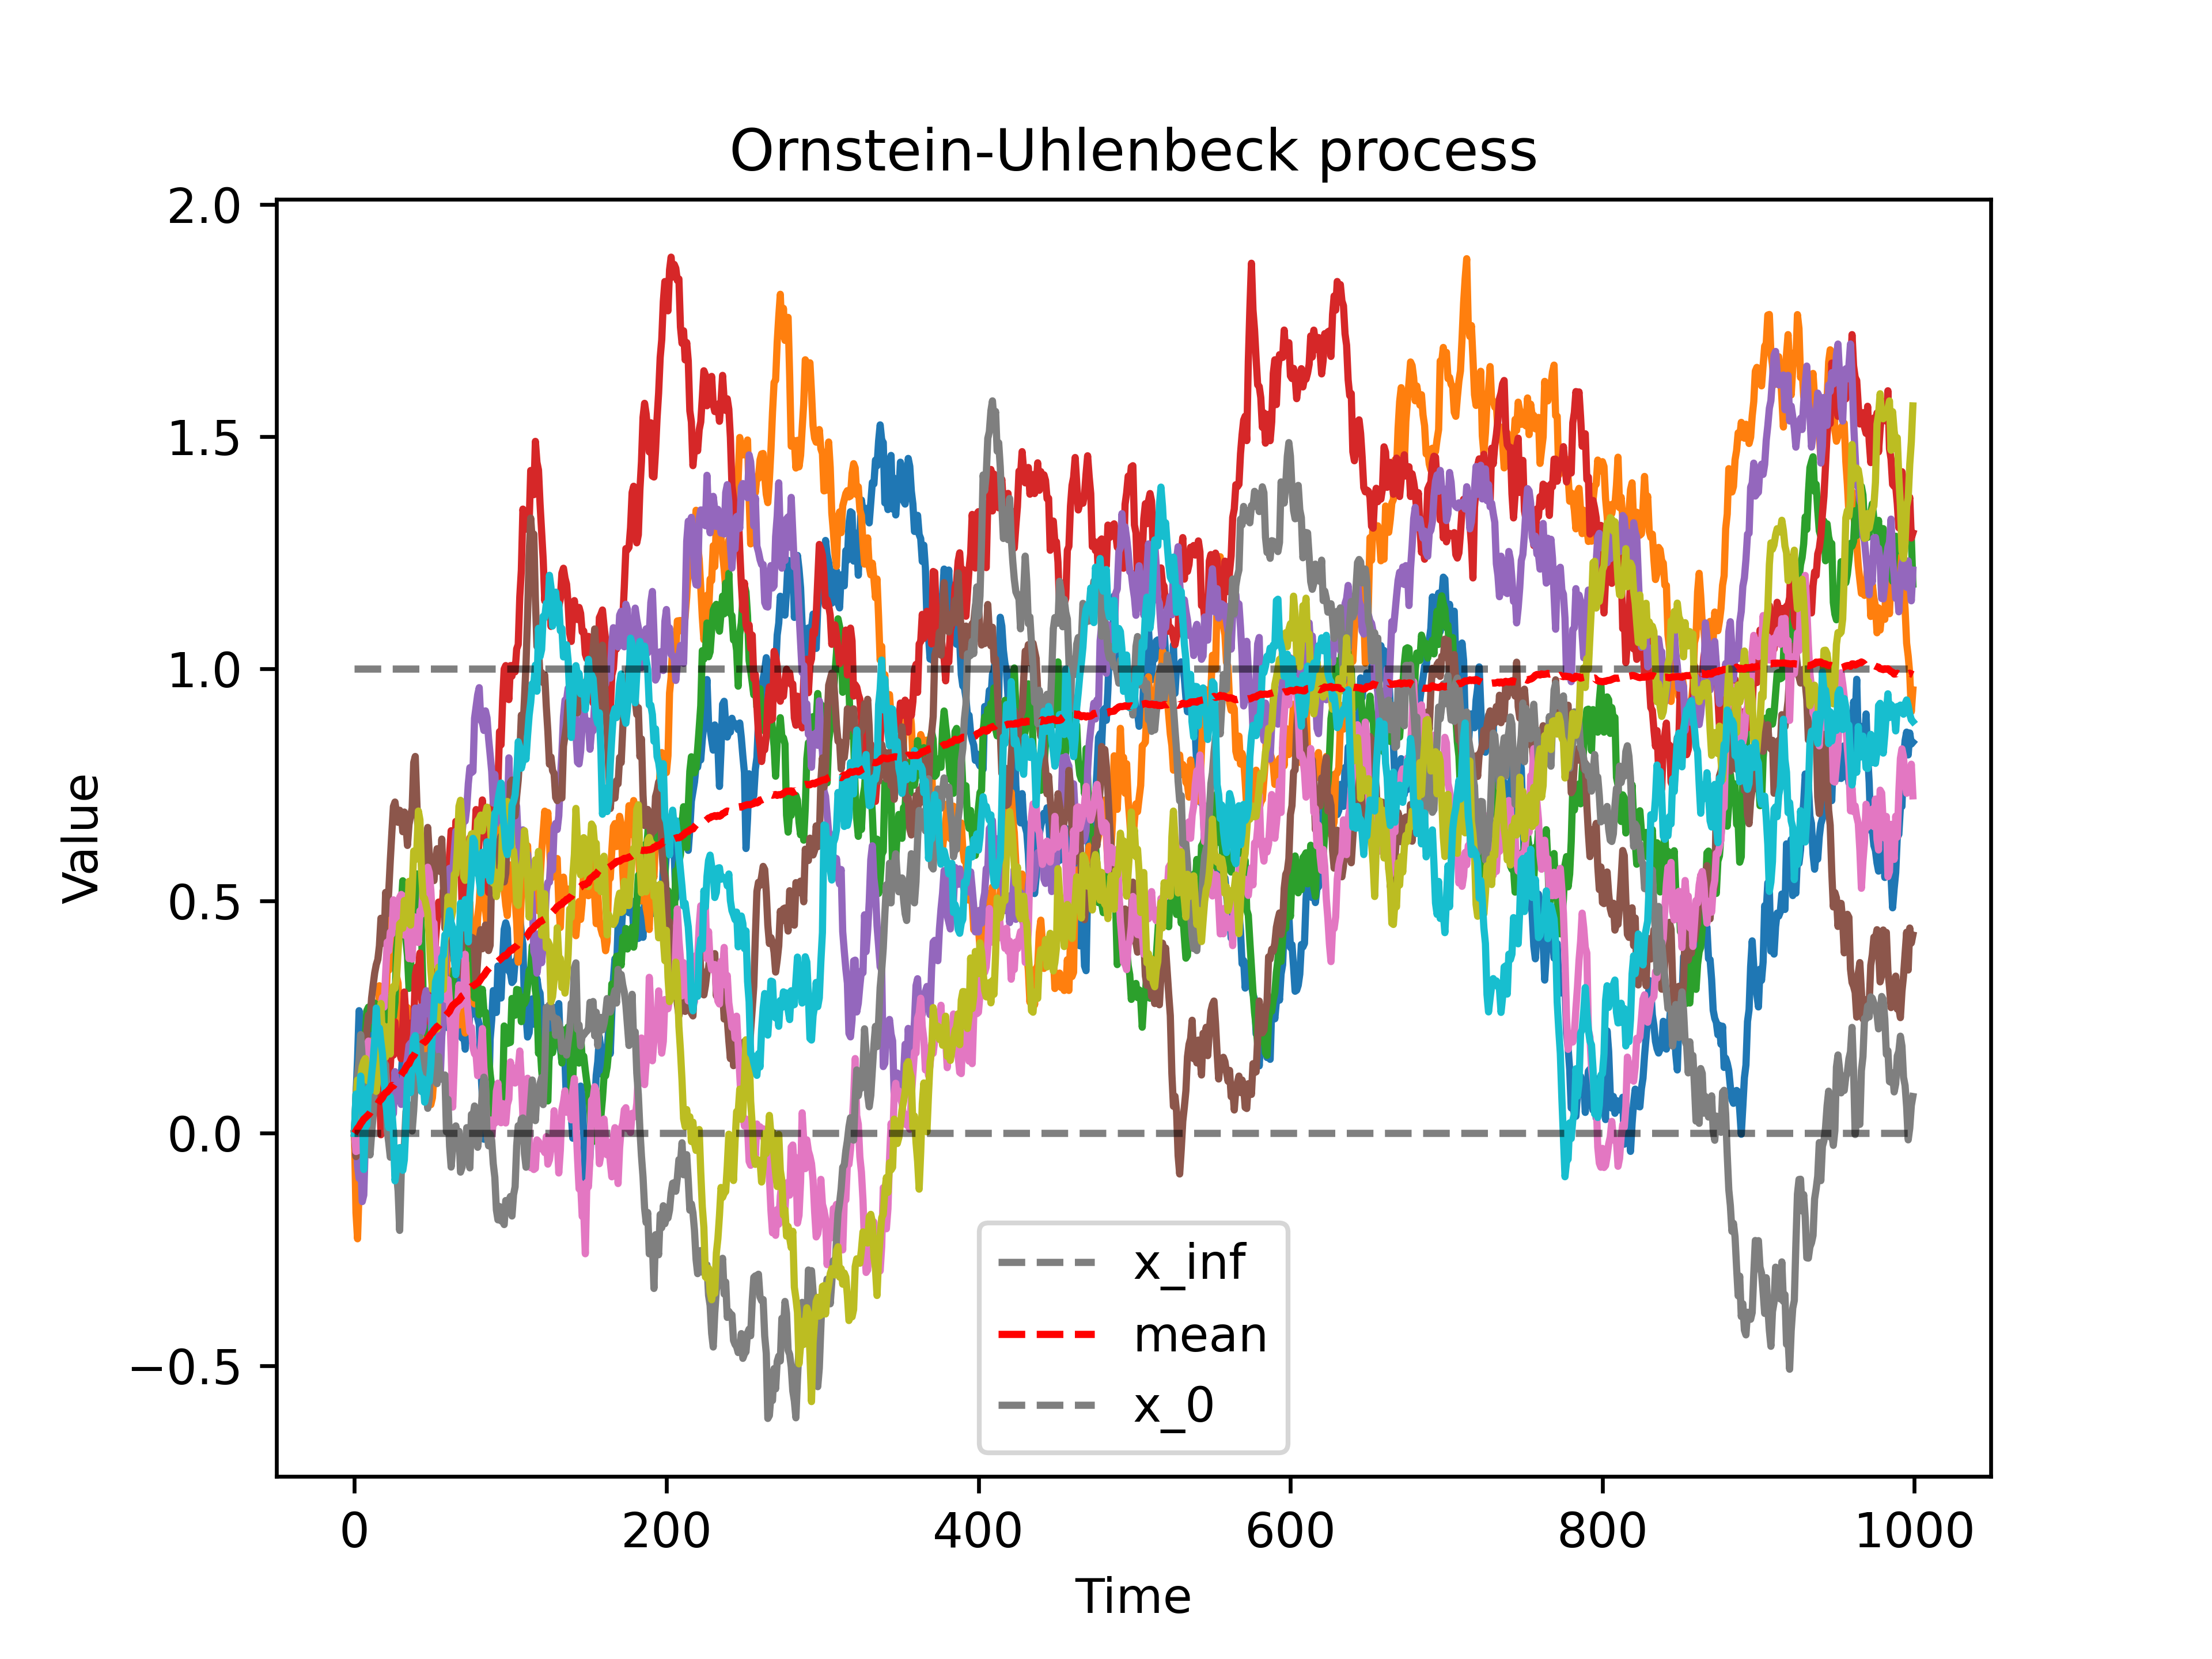
\includegraphics[width=1\textwidth]{plots/ou_process.png} % Replace 'example-image' with the filename of your image
    \caption{Plot showing some sample paths from the OU process, their mean and the \(x_\infty \) .}
    \label{fig:my_image}
\end{figure}

Regarding the variance, we plot in \ref{fig:covariance} the theoretical variance as well as the numeric one.


\begin{figure}[h!]
    \centering
    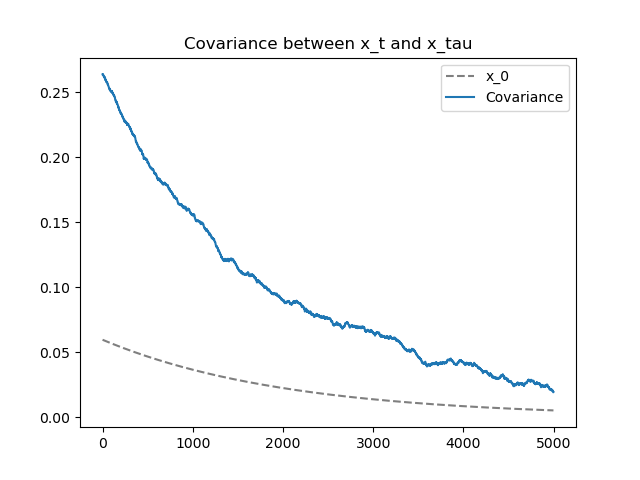
\includegraphics[width=1\textwidth]{plots/covariance.png} % Replace 'example-image' with the filename of your image
    \caption{Plot showing the covariance between \(X_t\) and \(X_{t+\tau } \) for \(\tau >0\).}
    \label{fig:covariance}
\end{figure}




\end{document}